\documentclass{beamer}
\usepackage{graphicx}
\begin{document}
\title{Array-Based Topological Mesh Representation
 Supporting General Modification}
\author{Dan Ibanez}

\frame{\titlepage}

\frame{\frametitle{Overview}
SCOREC has developed a mesh data structure with
the following features:
\begin{itemize}
\item composed of several large arrays
\item addition and removal are $O(1)$ operations
\item supports mixed element types
\item can represent parallel meshes
\item stores arbitrary associated data
\item uses 4x less memory than current structures
\end{itemize}
}

\frame{\frametitle{Basic Mesh Data Structure}
The simplest mesh data structure is an element to
node connectivity array.

Given an integer element id, returns the integer
node ids of that element.

Sufficient for element integration, element
stiffness matrix assembly, etc.

\vskip 20pt

\begin{center}
\includegraphics{ibanez_cse15-1.eps}
\hspace{30pt}
\includegraphics{ibanez_cse15-2.eps}
\end{center}
}

\frame{\frametitle{Adjacency Graph}
Element to node connectivity forms a bipartite graph
where all elements of the same topological type
have the same degree.

In the example, both elements are quadrilaterals.

\begin{center}
\includegraphics{ibanez_cse15-3.eps}
\end{center}
}

\frame{\frametitle{Upward Adjacency}
The inverse of element-node connectivity, i.e.
which elements are adjacent to a node.

This is harder, because the degrees are not the same.

Object-based structures may store many small arrays.

\begin{center}
\includegraphics{ibanez_cse15-4.eps}
\end{center}

Required during any kind of mesh modification, including
element load balancing.
}

\frame{\frametitle{Compact Upward Adjacency}
Assuming a mesh is static, the upward data
can be placed in one array.

Note that it is exactly the same size as the downward
array.

That is because {\emph each entry represents an adjacency
graph edge}, in both arrays.

\begin{center}
\includegraphics{ibanez_cse15-5.eps}
\end{center}
}

\frame{\frametitle{Linked Upward Adjacency}
We can also rearrange the entries of the upward array
to match the ordering of the downward array, such
that the same graph edge has the same index.

\begin{center}
\includegraphics{ibanez_cse15-6.eps}
\end{center}

Element id is now implicit by location, but
entries are non-contiguous and must be linked.
}

\frame{\frametitle{Upward Adjacency Arrays}
Since the element id can be derived from the entry's
position, we can use the entries to store list links
instead.
Another array for the nodes points to the head
of the list.

\begin{center}
\includegraphics{ibanez_cse15-7.eps}
\end{center}

Array indices are used instead of pointers.
Upward adjacency can still be derived by traversing
these lists-in-arrays.
}

\frame{\frametitle{Upward Adjacency Rationale}
Why use this complex lists-in-arrays structure to encode
upward adjacency ?

\begin{enumerate}
\item very compact storage
\item elements can be added and removed more easily
\item indices use less memory than pointers
\end{enumerate}
}

\frame{\frametitle{Mesh Modification}
All mesh modification can be implemented as element
addition and removal.

We have arrays of size $CN$ where $N$ is the
number of entities of one type, and entries
$[Ci, C(i + 1) - 1]$ correspond to entity $i$.

We need general array modification algorithms
for adding and removing entries
(or contiguous $C$ entries).
}

\frame{\frametitle{Array Addition}
\begin{itemize}
\item
Common solution is geometric growth with additions to the end.
For example, C++ std::vector uses this algorithm.
\item
Array has allocated capacity $(c)$ and used size.
When addition is requested and used size equals capacity,
reallocate to capacity $\alpha c$.
We use $\frac32(c+1)$.
\item
Result is amortized $O(1)$ addition runtime.
\item
C's realloc is more efficient due
to mmap on Linux systems.
\end{itemize}
\begin{center}
\includegraphics{ibanez_cse15-9.eps}
\end{center}
}

\frame{\frametitle{Array Removal}
\begin{itemize}
\item
Removal can happen anywhere, leaves a hole.
\item
Trying to fill the hole requires moving another
entry or entries
\item
But changing indices is bad for users, they
need unique consistent identifiers
\item
So, keep the holes and track them
\end{itemize}
}

\frame{\frametitle{Free List}
\begin{itemize}
\item
Another array, this one tracks holes
\item
Holes are linked together in to one ``free list".
\item
On removal, new hole is linked to front of list.
\item
On addition, check for holes and if so unlink
the first hole from the list and fill it.
\end{itemize}

\begin{center}
\includegraphics{ibanez_cse15-8.eps}
\end{center}
}

\frame{\frametitle{Array Modification Algorithm}
On removal, link new hole into free list.

On addition:
\begin{enumerate}
\item
If there are holes, unlink the first hole
and return its index
\item
If used size equals capacity, reallocate for
bigger capacity
\item
Increment used size, return last index
\end{enumerate}

This logic is applied to all arrays associated
with that entity type: downward adjacency,
upward adjacency, and the free list array itself.
}

\frame{\frametitle{Element-Node Structure}
\begin{itemize}
\item nodal free list array
\item element free list array
\item element to node array
\item node to element arrays (2)
\item additional fields, indexed by node id
\end{itemize}
}

\frame{\frametitle{Full Topological Representation}
\begin{columns}[T]
\begin{column}{0.4\textwidth}
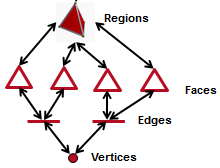
\includegraphics[width=\textwidth]{full.png}
\end{column}
\begin{column}{0.6\textwidth}
\begin{itemize}
\item Each dimension explicitly represented
\item Adjacency between each pair of dimensions
\item Uses
\begin{itemize}
\item Faces for bounday conditions
\item Edge-driven mesh adaptation
\item Better parallel decoupling
\end{itemize}
\end{itemize}
\end{column}
\end{columns}
}

\frame{\frametitle{Full Topological Structure}
\begin{itemize}
\item free list array per dimension (4)
\item downward array per dimension (3)
\item upward arrays per dimension (6)
\item additional fields, indexed by entity id
\end{itemize}
Operations
\begin{itemize}
\item Add entity and set one-level up/down adjacencies
\item Remove entity
\item Query one-level upward adjacency
\item Query one-level downward adjacency
\item Iterate (increment, skip holes)
\end{itemize}
}

\frame{\frametitle{Mixed Meshes}
\begin{itemize}
\item Multiple topological types per dimension
\item Each per-dimension array is split into
per-type arrays
\item 2D array indices are encoded as $e = iT + t$,
where $T$ is the number of types, $t$ is entity type,
$i$ is index in array.
\item this applies to downward arrays, upward list arrays,
and additional field arrays.
\end{itemize}

\begin{center}
\includegraphics{ibanez_cse15-10.eps}
\end{center}
}

\frame{\frametitle{Memory Use}
94K tet mesh including coordinates,
geometric classification, and matched faces.

\begin{center}
\begin{tabular}{lrrr}
library & MB & bytes per tet & relative \\\hline
pumi & 84.1 & 897 & 100\% \\
simmetrix  & 55.2 & 589 &  66\% \\
mds  & 22.6 & 241 &  27\% \\
\end{tabular}
\end{center}
}

\end{document}
